\chapter{Experiments} % (fold)
\label{cha:experiments}
    In this final chapter we present the results we obtained by applying our model to the datasets we have used
    to validate and test our ANN, namely, MONKS and CUP. Other than the results, we also present some details
    about the validation phase for each one of the datasets. In appendix \ref{cha:monks_learning_curves} and
    \ref{cha:cup_learning_curves} we added some graphs of the ANN's performances during the experimental phases, in
    order to enrich the presentation.

    \section{MONKS} % (fold)
    \label{sec:monks}
        Before delving into the details of the results we obtained by applying our model to the dataset, we
        provide some informations about the \textit{preprocessing routines} and \textit{validation schema} we
        decided to use. Here are the steps we followed in order to reach the final states of our analysis.

        \begin{enumerate}
            \item Since the MONKS datasets’ feature are categorical, that is, every feature’s value represents
            a class, not a numerical value, we preprocessed the three datasets by writing a script
            for applying a \textit{1-of-k encoding}, hence obtaining 17 binary input features.
            \item As a supplementary preprocessing phase, we have applied a \textit{symmetrization} to the
            matrix containing the dataset’s values, in order to ease the training during the validation phase
            by having a matrix of values closer to the symmetric behavior of the sigmoid function, which was
            introduced in section \ref{sec:the_activation_functions}.
            \item Since we have chosen to follow \cite{Bergstra:2012:RSH:2188385.2188395} for the
            hyperparameters' search during the validation phase, we first performed some
            \textit{preliminary trials} in order to have a glimpse on the best intervals for searching our
            model's hyperparameters. During this trials we manually varied the model's hyperparameters, e.g.
            the learning rate, the momentum constant and so on for the SGD and the rho constant for the CGD,
            and observed the resulting \textit{learning curves}. For this part of the analysis we have used
            the $20\%$ of the training set as validation set, and the remaining part for training the network.
            \item We then deepen the search using the most interesting intervals discovered during the
            preliminary trials in the validation phase by using our implementation of the (random)
            \textit{grid search algorithm}, in which we also used our implementation of the
            \textit{k-fold cross validation algorithm} (which follows the approach of using a value
            of 5 for the k parameter).
        \end{enumerate}

        Our validation schema for the MONKS dataset essentially consists in using the random grid
        search algorithm to investigate some random sampled "points" in the hyperparameters' space, evaluating
        the performances for each one of this points and finally selecting the best combinations of parameters
        based on the diffent metrics like \textit{generalization error}, \textit{accuracy}, \textit{precision},
        \textit{recall} and \textit{f1-score}. In Tab. \ref{tab:hyper_monk} are reported the ranges for the
        hyperparameters involved in the validation phase.

        \begin{table}[H]
          \centering
          \caption{Hyperparameters' ranges for the random grid search algorithm with SGD and CG.}
          \begin{minipage}{.4\textwidth}
              \centering
              \begin{tabular}{| c | c |}
                    \hline
                    Hyperparameters & Ranges\\
                    \hline
                    $\eta$ & $\left [0.6, 0.8 \right ]$ \\
                    \hline
                    $\alpha$ & $[0.5, 0.9]$ \\
                    \hline
                    $\lambda$ & $[0.001, 0.01]$ \\
                    \hline
              \end{tabular}
          \end{minipage}
          \begin{minipage}{.4\textwidth}
              \centering
              \begin{tabular}{| c | c |}
                    \hline
                    Hyperparameters & Ranges\\
                    \hline
                    $\sigma_2$ & $\left [0.1, 0.4 \right ]$ \\
                    \hline
                    $\rho$ & $[0.0, 1.0]$ \\
                    \hline
              \end{tabular}
            \end{minipage}
            \label{tab:hyper_monk}
        \end{table}

        In order to compare the
        results in a similar configuration between the SGD and the CG, we have decided to adopt only the \textit{batch} mode for training the ANN. 
            % The regularization constant $\lambda$ is used only in
            % the third dataset, since Monk 3 is the only one among the three that has noisy samples. 

        In the following tables, the tasks are divided by the kind of dataset that has been used during the iteration, and, for
        each one of the tasks, the network's topology is the same, that is, 17 -> 4 -> 8 -> 1.

        For each
        task, the results concerning the MSE and the accuracy are collected by taking the mean of the
        output of 10 different iterations. In gray we can see the best optimizer for each one of the
        tasks. We added some additional statistics
        regarding the execution times in milliseconds of the various iterations. As for the other table, the best
        optimizers for each of the tasks are colored in gray.

        \subsection{Results (no max epochs)} % (fold)
        \label{sub:results_}

            In order to compare the behaviour of the different algorithms with a focus on the  optimization, the accuracy, in term of the final value taken by norm of the gradient, has been set to $10^{-3}$. 

            All the methods have been trained with the same hyperparameters, and the only stopping criteria that has been chosen is the decreasing of the norm.

            \begin{table}[H]
                \centering
                \begin{subtable}{\textwidth}
                    \resizebox{\textwidth}{!}{
                        \begin{tabular}{| c | c | c | c | c | c | c | c | c | c |}
                            \hline
                            Task &  Optimizer &  $\sigma_1$ &  $\sigma_2$ &   $\rho$ &   $\eta$ &  $\alpha$ &  $\lambda$ &        MSE (TR - TS) &   Accuracy (TR - TS) (\%) \\
                            \hline
                            \rowcolor[gray]{.9}
                            MONK 1 &   SGD (CM) &        - &        - &     - &  0.61 &   0.83 &  0.0 &  1.00e-05 - 9.64e-06 &  100 \% - 100 \% \\
                            \hline
                            MONK 1 &  SGD (NAG) &        - &        - &     - &  0.61 &   0.83 &  0.0 &  1.39e-05 - 1.28e-05 &  100 \% - 100 \% \\
                            \hline
                            MONK 1 &   CGD (PR) &   0.0001 &     0.3 &  0.0 &     - &      - &       - &  6.11e-03 - 2.00e-02 &  99 \% - 96 \% \\
                            \hline
                            MONK 1 &   CGD (HS) &   0.0001 &     0.3 &  0.0 &     - &      - &       - &  6.11e-03 - 2.00e-02 &  99 \% - 96 \% \\
                            \hline
                            MONK 1 &  CGD (MHS) &   0.0001 &     0.3 &  0.67 &     - &      - &       - &  1.49e-05 - 1.43e-05 &  100 \% - 100 \% \\
                            \hline
                            \hline
                            MONK 2 &   SGD (CM) &        - &        - &     - &  0.61 &   0.83 &  0.0 &  7.56e-06 - 7.37e-06 &  100 \% - 100 \% \\
                            \hline
                            MONK 2 &  SGD (NAG) &        - &        - &     - &  0.61 &   0.83 &  0.0 &  9.27e-06 - 9.82e-06 &  100 \% - 100 \% \\
                            \hline
                            MONK 2 &   CGD (PR) &   0.0001 &     0.3 &  0.0 &     - &      - &       - &  8.41e-06 - 5.97e-06 &  100 \% - 100 \% \\
                            \hline
                            MONK 2 &   CGD (HS) &   0.0001 &     0.3 &  0.0 &     - &      - &       - &  8.38e-06 - 6.33e-06 &  100 \% - 100 \% \\
                            \hline
                            \rowcolor[gray]{.9}
                            MONK 2 &  CGD (MHS) &   0.0001 &     0.3 &  0.67 &     - &      - &       - &  5.91e-06 - 5.72e-06 &  100 \% - 100 \% \\
                            \hline
                            \hline
                            MONK 3 &   SGD (CM) &        - &        - &     - &  0.61 &   0.83 &  0.0 &  2.07e-03 - 3.87e-06 &  97 \% - 100 \% \\
                            \hline
                            MONK 3 &  SGD (NAG) &        - &        - &     - &  0.61 &   0.83 &  0.0 &  1.78e-06 - 2.40e-06 &  100 \% - 100 \% \\
                            \hline
                            \rowcolor[gray]{.9}
                            MONK 3 &   CGD (PR) &   0.0001 &     0.3 &  0.0 &     - &      - &       - &  1.43e-06 - 1.50e-06 &  100 \% - 100 \% \\
                            \hline
                            MONK 3 &   CGD (HS) &   0.0001 &     0.3 &  0.0 &     - &      - &       - &  6.20e-03 - 1.43e-06 &  99 \% - 100 \% \\
                            \hline
                            MONK 3 &  CGD (MHS) &   0.0001 &     0.3 &  0.67 &     - &      - &       - &  1.24e-02 - 3.80e-06 &  98 \% - 100 \% \\
                            \hline
                        \end{tabular}
                    }
                \end{subtable}
                \caption{Comparisons between the iterations having no maximal number of epochs. Each one of the
                iterations has been completed with a network having topology 17 -> 4 -> 8 -> 1.}
                \label{tab:monks_no_max_epochs}
            \end{table}

            \begin{table}[H]
                \centering
                \begin{subtable}{\textwidth}
                    \resizebox{\textwidth}{!}{
                        \begin{tabular}{| c | c | c | c | c | c | c | c |}
                            \toprule
                               Task &  Optimizer & Convergence Epoch &  LS Iterations &  Elapsed Time &   BP Time &   LS Time &  Dir Time \\
                            \hline
                             MONK 1 &   SGD (CM) &             25829 &              - &      80835.78 &   6097.73 &         - &         - \\
                            \hline
                             MONK 1 &  SGD (NAG) &             14382 &              - &      44410.24 &   3271.03 &         - &         - \\
                            \hline
                             MONK 1 &   CGD (PR) &               806 &            8.0 &       9728.46 &   1364.61 &   5750.07 &     15.10 \\
                            \hline
                             MONK 1 &   CGD (HS) &               770 &            8.0 &       9468.09 &   1324.35 &   5595.54 &     14.52 \\
                            \hline
                            \rowcolor[gray]{.9}
                             MONK 1 &  CGD (MHS) &               472 &            8.0 &       5307.14 &    749.90 &   3151.04 &      7.26 \\
                            \hline
                            \hline
                             MONK 2 &   SGD (CM) &             14586 &              - &      56437.37 &   3906.62 &         - &         - \\
                            \hline
                             MONK 2 &  SGD (NAG) &              7743 &              - &      28037.07 &   1887.81 &         - &         - \\
                            \hline
                            \rowcolor[gray]{.9}
                             MONK 2 &   CGD (PR) &               292 &            8.0 &       3944.34 &    579.52 &   2236.75 &      5.01 \\
                            \hline
                             MONK 2 &   CGD (HS) &               340 &            8.0 &       4385.45 &    650.30 &   2479.65 &      5.45 \\
                            \hline
                             MONK 2 &  CGD (MHS) &               513 &            8.0 &       6567.70 &    967.88 &   3769.13 &      8.12 \\
                            \hline
                            \hline
                             MONK 3 &   SGD (CM) &             65306 &              - &     175429.15 &  13298.60 &         - &         - \\
                            \hline
                             MONK 3 &  SGD (NAG) &             50918 &              - &     163439.49 &  12167.22 &         - &         - \\
                            \hline
                             MONK 3 &   CGD (PR) &              6540 &            8.0 &      74283.88 &  10581.14 &  44239.27 &    109.15 \\
                            \hline
                             MONK 3 &   CGD (HS) &              4056 &            8.0 &      50295.56 &   7223.92 &  29842.22 &     75.06 \\
                            \hline
                            \rowcolor[gray]{.9}
                             MONK 3 &  CGD (MHS) &              2209 &            8.0 &      23903.49 &   3417.29 &  14174.89 &     32.84 \\
                            \hline
                            \end{tabular}

                    }
                \end{subtable}
                \caption{Additional time-related statistics. The unit of time that has been used is the
                millisecond.}
                \label{tab:monks_additional_no_max_epochs}
            \end{table}

            In Table \ref{tab:monks_no_max_epochs} and \ref{tab:monks_additional_no_max_epochs}   we can find the results for the iterations completed without
            constraining the optimizers by imposing a maximal number of epochs of training.

            It's immediately evident the different number of iterations that the Conjugate Gradient methods and the Stochastic Gradient Descent need in order to converge to the imposed threshold.

            As we can expect from the theory, the CG methods are usually able to converge in the first 1000 iterations, while the SGD is extremely slower, needing more than 20000 iterations in order to arrive to the same level of accuracy.

            It's worth to notice that the all these methods have to face some limitations when dealing with a noisy dataset as Monks 3, even though each one of them still confirms their typical behaviour.
            
            Even when looking at the time of execution of the various algorithms, there is no surprise in the results. What is more interesting to underline is, as evident in the plots of Fig. \ref{fig:monks_MSE_all}, is the longer time needed by the SGD, even if a better performace is given by the use of the NAG momentum. 
            When comparing the plots, we can see that, even though the number of iterations of the CG methods is different, when taking into account the time of execution, some iterations are more costly than other. That means, some methods could need more time in computing the right weights updates, even if they could converge in a lower number of iterations. 

            Futhermore, the majority of the time (more than half of the time) is spent in computing the Line Search, which tipically needs to perform 8 iterations in order to find the right learning step.

            Taking into account also the accuracy in the prediction of the neural network, the $MHS^+$ methods is the one having an overall better behaviour.

            \begin{figure}[t!]{}
                \centering
                \begin{subfigure}{0.45\textwidth}
                    \resizebox{\textwidth}{!}{
                        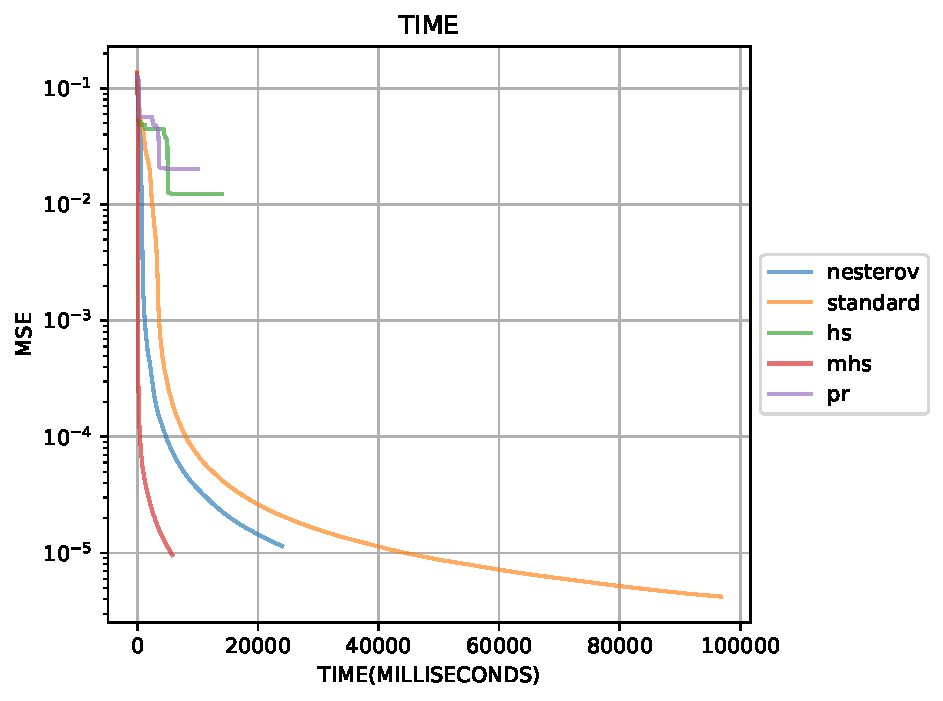
\includegraphics{img/analytics/1_mse_all_time.pdf}
                    }
                    \caption{}
                    \label{fig:monks_1_MSE_all_t}
                \end{subfigure}
                \begin{subfigure}{0.45\textwidth}
                    \resizebox{\textwidth}{!}{
                        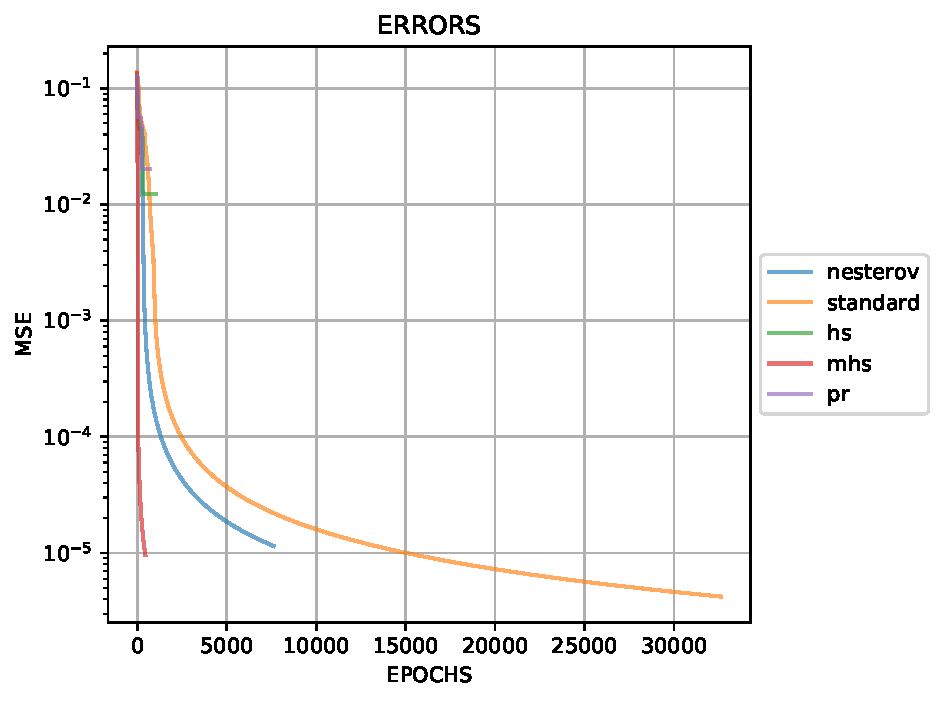
\includegraphics{img/analytics/1_mse_all.pdf}
                    }
                    \caption{}
                    \label{fig:monks_1_MSE_all}
                \end{subfigure}
                \begin{subfigure}{0.45\textwidth}
                    \resizebox{\textwidth}{!}{
                        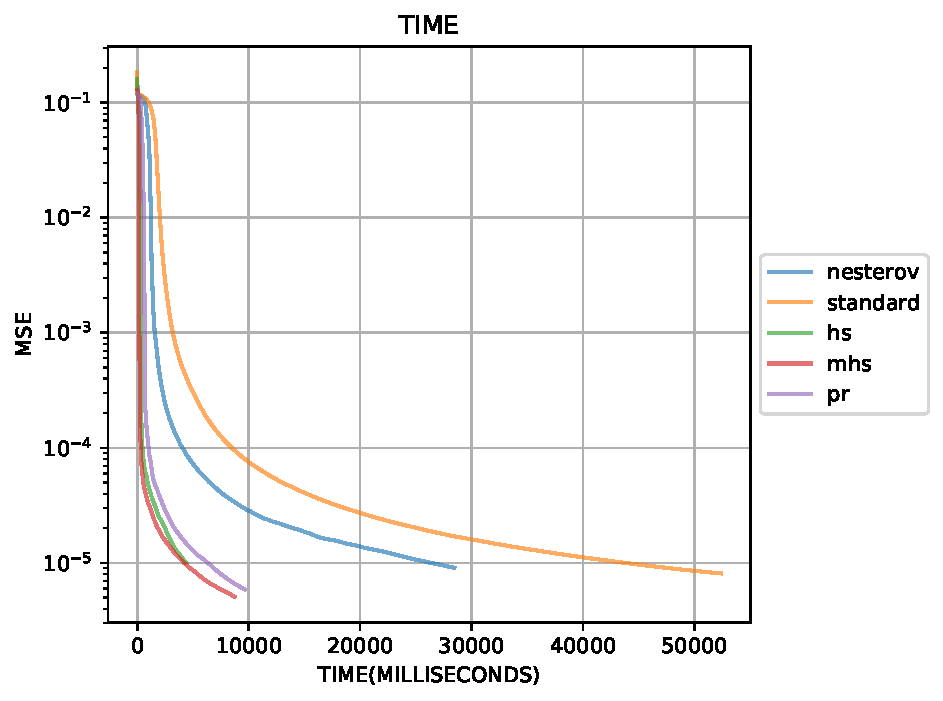
\includegraphics{img/analytics/2_mse_all_time.pdf}
                    }
                    \caption{}
                    \label{fig:monks_2_MSE_all_t}
                \end{subfigure}
                \begin{subfigure}{0.45\textwidth}
                    \resizebox{\textwidth}{!}{
                        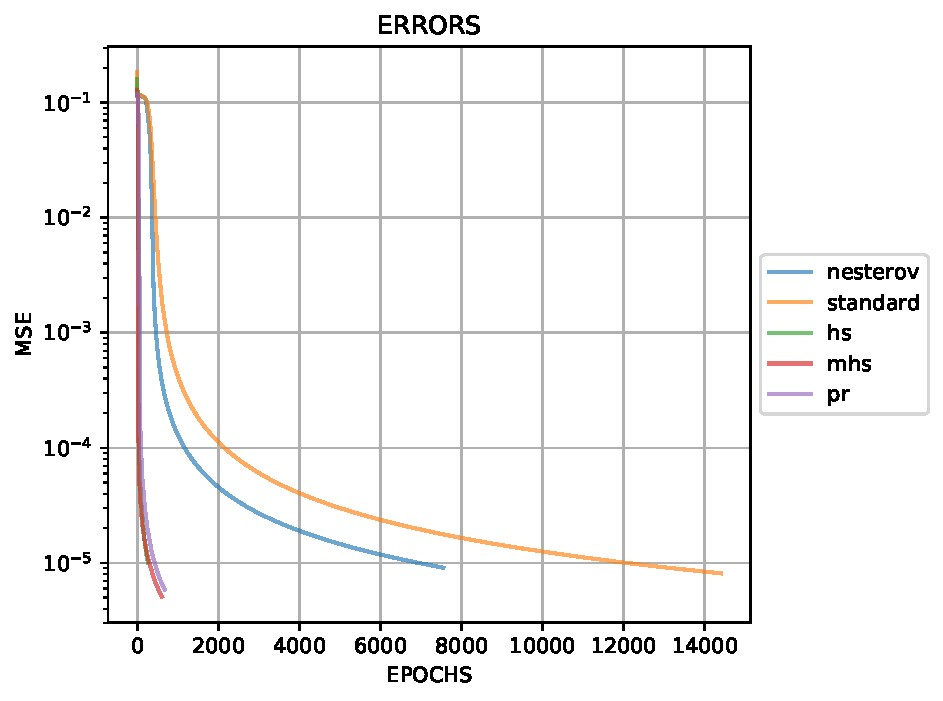
\includegraphics{img/analytics/2_mse_all.pdf}
                    }
                    \caption{}
                    \label{fig:monks_2_MSE_all}
                \end{subfigure}
                \begin{subfigure}{0.45\textwidth}
                    \resizebox{\textwidth}{!}{
                        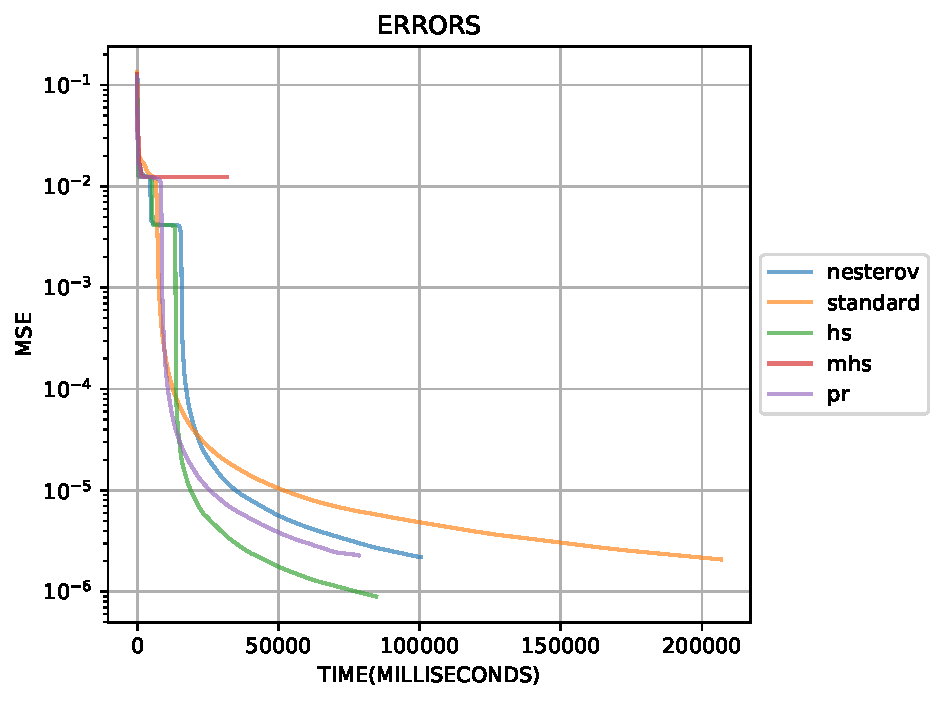
\includegraphics{img/analytics/3_mse_all_time.pdf}
                    }
                    \caption{}
                    \label{fig:monks_3_MSE_all_t}
                \end{subfigure}
                \begin{subfigure}{0.45\textwidth}
                    \resizebox{\textwidth}{!}{
                        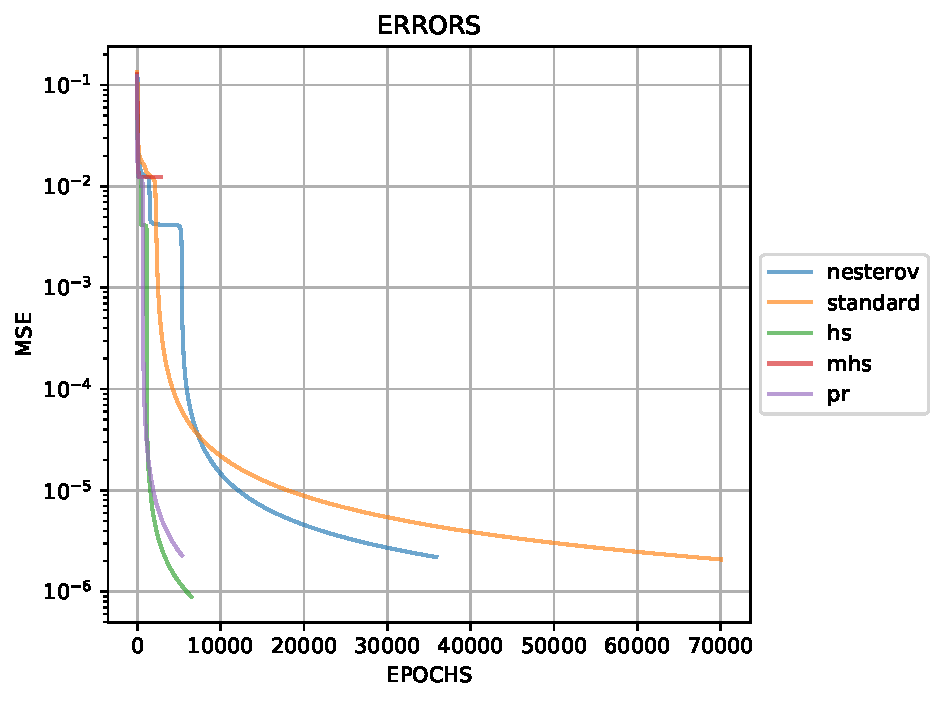
\includegraphics{img/analytics/3_mse_all.pdf}
                    }
                    \caption{}
                    \label{fig:monks_3_MSE_all}
                \end{subfigure}
                \caption{Comparisons between the different optimizers without the constrain of setting a maximal
                number of epochs for the iterations. In Figure \ref{fig:monks_1_MSE_all}, \ref{fig:monks_1_MSE_all_t} we can see the
                comparison for MONKS 1, while in Figure \ref{fig:monks_2_MSE_all}, \ref{fig:monks_2_MSE_all_t} we can see the one for
                MONKS 2 and finally in Figure \ref{fig:monks_3_MSE_all},  \ref{fig:monks_3_MSE_all_t} we can see the one for MONKS 3.}
                \label{fig:monks_MSE_all}
            \end{figure}

        % subsection results_ (end)

        \subsection{Results (max epochs 1000)} % (fold)
        \label{sub:results_}

            \begin{table}[H]
                \centering
                \begin{subtable}{\textwidth}
                    \resizebox{\textwidth}{!}{
                        \begin{tabular}{| c | c | c | c | c | c | c | c | c | c |}
                            \hline
                             Task &  Optimizer &  $\sigma_1$ &  $\sigma_2$ &   $\rho$ &   $\eta$
                             &  $\alpha$ &  $\lambda$ & MSE (TR - TS) &   Accuracy (TR - TS) (\%) \\
                             \hline
                            MONK 1 &   SGD (CM) &        - &        - &     - &  0.65 &   0.75 &  0.0 &  9.92e-03 - 1.48e-02 &  99 \% - 99 \% \\
                            \hline
                            MONK 1 &  SGD (NAG) &        - &        - &     - &  0.63 &   0.73 &  0.0 &  2.18e-02 - 3.17e-02 &  97 \% - 96 \% \\
                            \hline
                            MONK 1 &   CGD (PR) &   0.0001 &     0.18 &  0.0 &     - &      - &       - &  1.54e-02 - 4.88e-02 &  97 \% - 90 \% \\
                            \hline
                            \rowcolor[gray]{.9}
                            MONK 1 &   CGD (HS) &   0.0001 &     0.22 &  0.0 &     - &      - &       - &  2.12e-03 - 9.71e-03 &  100 \% - 98 \% \\
                            \hline
                            MONK 1 &  CGD (MHS) &   0.0001 &     0.13 &  0.86 &     - &      - &       - &  8.97e-03 - 1.92e-02 &  98 \% - 96 \% \\
                            \hline
                            \hline
                            \rowcolor[gray]{.9}
                            MONK 2 &   SGD (CM) &        - &        - &     - &  0.71 &   0.89 &  0.0 &  6.99e-03 - 9.65e-03 &  100 \% - 100 \% \\
                            \hline
                            MONK 2 &  SGD (NAG) &        - &        - &     - &  0.64 &   0.85 &  0.0 &  1.34e-02 - 1.91e-02 &  98 \% - 98 \% \\
                            \hline
                            MONK 2 &   CGD (PR) &   0.0001 &     0.34 &  0.0 &     - &      - &       - &  1.59e-02 - 3.86e-02 &  96 \% - 92 \% \\
                            \hline
                            MONK 2 &   CGD (HS) &   0.0001 &     0.17 &  0.0 &     - &      - &       - &  1.06e-02 - 1.43e-02 &  98 \% - 97 \% \\
                            \hline
                            MONK 2 &  CGD (MHS) &   0.0001 &     0.33 &  0.43 &     - &      - &       - &  4.53e-03 - 1.13e-02 &  99 \% - 98 \% \\
                            \hline
                            \hline
                            MONK 3 &   SGD (CM) &        - &        - &     - &  0.67 &   0.85 &  0.0027 &  1.18e-02 - 1.31e-02 &  98 \% - 98 \% \\
                            \hline
                            MONK 3 &  SGD (NAG) &        - &        - &     - &  0.61 &   0.80 &  0.0036 &  1.67e-02 - 1.98e-02 &  97 \% - 97 \% \\
                            \hline
                            MONK 3 &   CGD (PR) &   0.0001 &     0.19 &  0.0 &     - &      - &       - &  2.07e-02 - 3.51e-02 &  94 \% - 93 \% \\
                            \hline
                            MONK 3 &   CGD (HS) &   0.0001 &     0.36 &  0.0 &     - &      - &       - &  9.03e-03 - 1.95e-02 &  98 \% - 96 \% \\
                            \hline
                            \rowcolor[gray]{.9}
                            MONK 3 &  CGD (MHS) &   0.0001 &     0.34 &  0.42 &     - &      - &       - &  7.01e-03 - 1.63e-02 &  99 \% - 96 \% \\
                            \hline
                        \end{tabular}
                    }
                \end{subtable}
                \caption{Comparisons between the iterations having a maximal number of epochs egual to 1000.
                Each one of the iterations has been completed with a network having topology
                17 -> 4 -> 8 -> 1.}
                \label{tab:monks_max_epochs}
            \end{table}

            \begin{table}[H]
                \centering
                \begin{subtable}{\textwidth}
                    \resizebox{\textwidth}{!}{
                        \begin{tabular}{| c | c | c | c | c | c | c | c |}
                            \toprule
                               Task &  Optimizer & Convergence Epoch &  LS Iterations &  Elapsed Time &  BP Time &  LS Time &  Dir Time \\
                            \hline
                             MONK 1 &   SGD (CM) &              1000 &              - &       5163.25 &   149.95 &        - &         - \\
                             \hline
                             MONK 1 &  SGD (NAG) &              1000 &              - &       5214.20 &   147.68 &        - &         - \\
                             \hline
                             MONK 1 &   CGD (PR) &               445 &            6.0 &       5055.85 &   514.70 &  2233.17 &     14.00 \\
                             \hline
                             \rowcolor[gray]{.9}
                             MONK 1 &   CGD (HS) &               240 &            6.0 &       2665.58 &   267.58 &  1164.87 &      7.95 \\
                             \hline
                             MONK 1 &  CGD (MHS) &               298 &            7.0 &       3278.08 &   328.36 &  1436.53 &      9.57 \\
                             \hline
                             \hline
                             MONK 2 &   SGD (CM) &              1000 &              - &       5385.27 &   159.47 &        - &         - \\
                             \hline
                             MONK 2 &  SGD (NAG) &              1000 &              - &       5437.32 &   157.63 &        - &         - \\
                             \hline
                             MONK 2 &   CGD (PR) &               326 &            5.0 &       3648.71 &   362.99 &  1603.26 &     10.17 \\
                             \hline
                             \rowcolor[gray]{.9}
                             MONK 2 &   CGD (HS) &               149 &            5.0 &       1695.45 &   169.52 &   760.82 &      4.90 \\
                             \hline
                             MONK 2 &  CGD (MHS) &               183 &            5.0 &       2023.54 &   198.10 &   892.13 &      5.83 \\
                             \hline
                             \hline
                             MONK 3 &   SGD (CM) &              1000 &              - &       5304.07 &   155.96 &        - &         - \\
                             \hline
                             MONK 3 &  SGD (NAG) &              1000 &              - &       5353.35 &   154.01 &        - &         - \\
                             \hline
                             \rowcolor[gray]{.9}
                             MONK 3 &   CGD (PR) &               371 &            5.0 &       4149.39 &   418.39 &  1821.40 &     11.66 \\
                             \hline
                             MONK 3 &   CGD (HS) &               377 &            6.0 &       4319.66 &   439.25 &  1891.85 &     12.75 \\
                             \hline
                             MONK 3 &  CGD (MHS) &               389 &            6.0 &       4361.18 &   438.78 &  1906.62 &     12.70 \\
                            \hline
                            \end{tabular}
                    }
                \end{subtable}
                \caption{Additional time-related statistics. The unit of time that has been used is the
                millisecond.}
                \label{tab:monks_additional_max_epochs}
            \end{table}

            Here we present the results from a series of iterations where the maximal number of epochs has
            been setted to 1000, in order to focus on a machine learning point of view. This time, the algorithms have been trained taking into account only the maximal number of epochs or the error goal=$10^{-4}$ for the CG methods.

            Similarly to the previous section, in Table \ref{tab:monks_max_epochs} we
            can find the details regarding the optimizers' performances, while in Table
            \ref{tab:monks_additional_max_epochs} there are the details regarding the time-related
            performances. The considerations done for the iterations with no maximal number of epochs are
            valid also for this specific case. In Figure \ref{fig:monks_MSE_all_max_epochs} we can see a
            comparison betweeen the various optimizers.

            In this case, it's more evident a behaviour introduced in the former experiments: in Monk 3, the CG methods and the SGD have spent a similar time of execution, even though the CG ones stopped in the first 300 iterations. 

            For what concernes the accuracy in the prediction, only few of the models get an accuracy of $100\%$, but it is still true that the CG gets very good results in a minor time of execution and in a minor number of iterations.

            \begin{figure}[t!]
                \centering
                \begin{subfigure}{0.45\textwidth}
                    \resizebox{\textwidth}{!}{
                        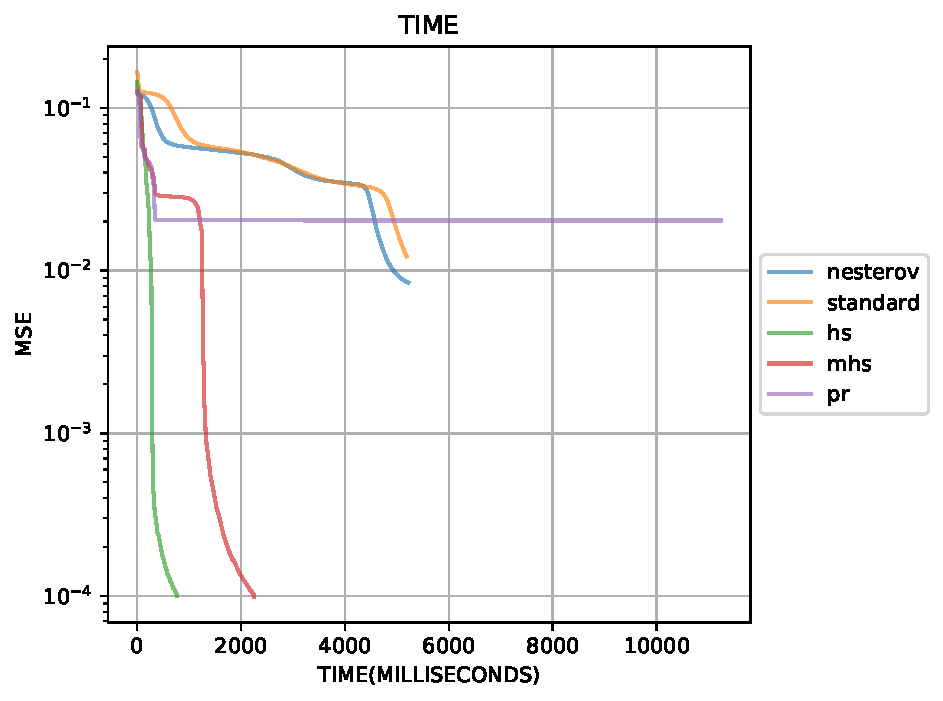
\includegraphics{img/comparisons/1_mse_all_time_max_epochs_1000.pdf}
                    }
                    \caption{}
                    \label{fig:monks_1_MSE_all_max_epochs_t}
                \end{subfigure}
                \begin{subfigure}{0.45\textwidth}
                    \resizebox{\textwidth}{!}{
                        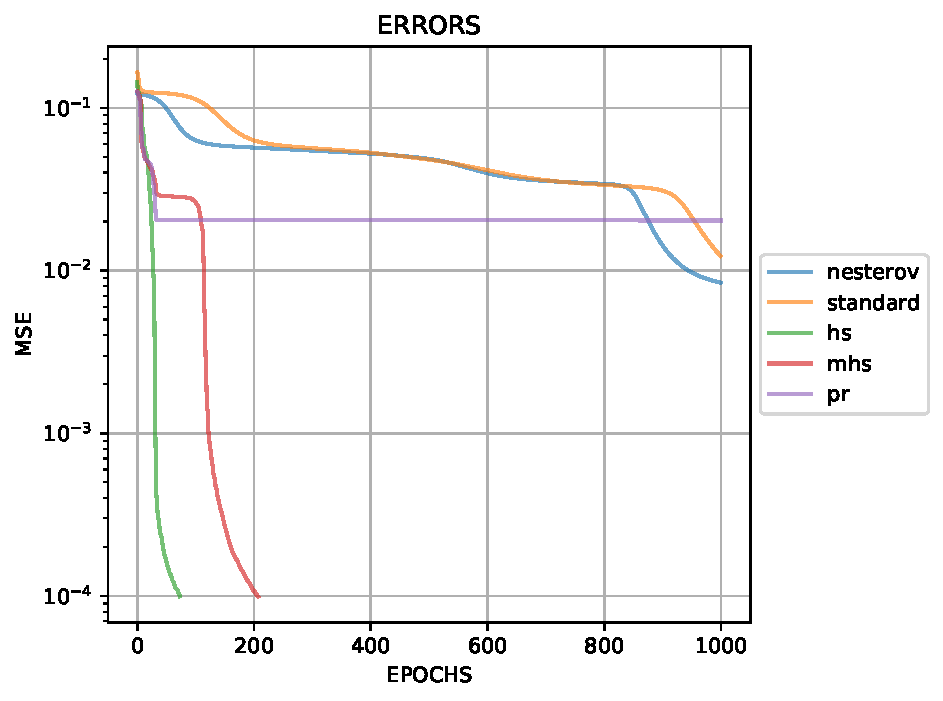
\includegraphics{img/comparisons/1_mse_all_max_epochs_1000.pdf}
                    }
                    \caption{}
                    \label{fig:monks_1_MSE_all_max_epochs}
                \end{subfigure}
                \begin{subfigure}{0.45\textwidth}
                    \resizebox{\textwidth}{!}{
                        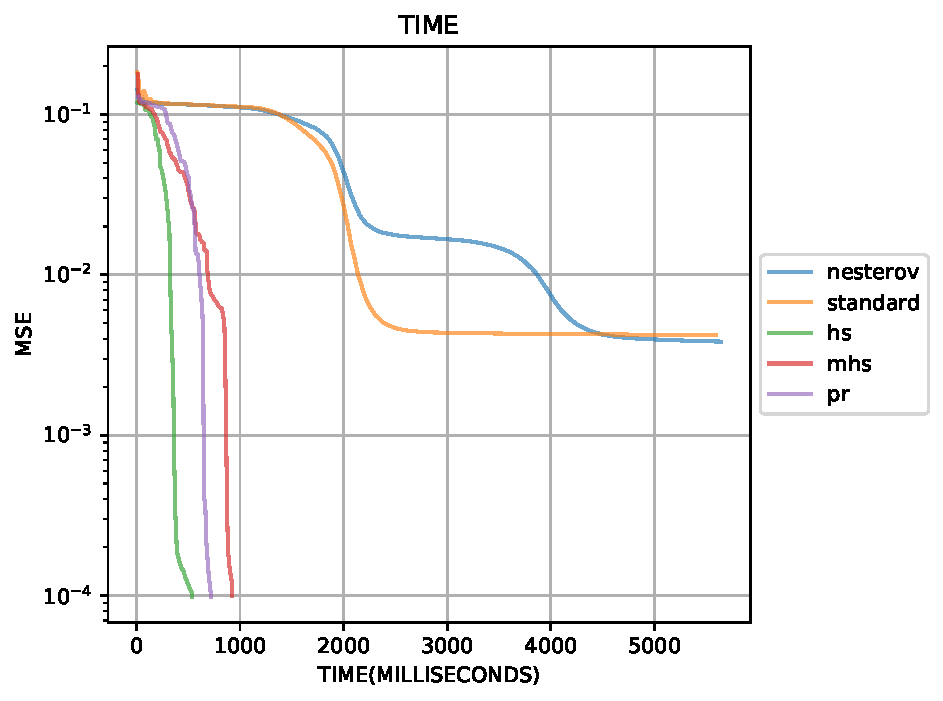
\includegraphics{img/comparisons/2_mse_all_time_max_epochs_1000.pdf}
                    }
                    \caption{}
                    \label{fig:monks_2_MSE_all_max_epochs_t}
                \end{subfigure}
                \begin{subfigure}{0.45\textwidth}
                    \resizebox{\textwidth}{!}{
                        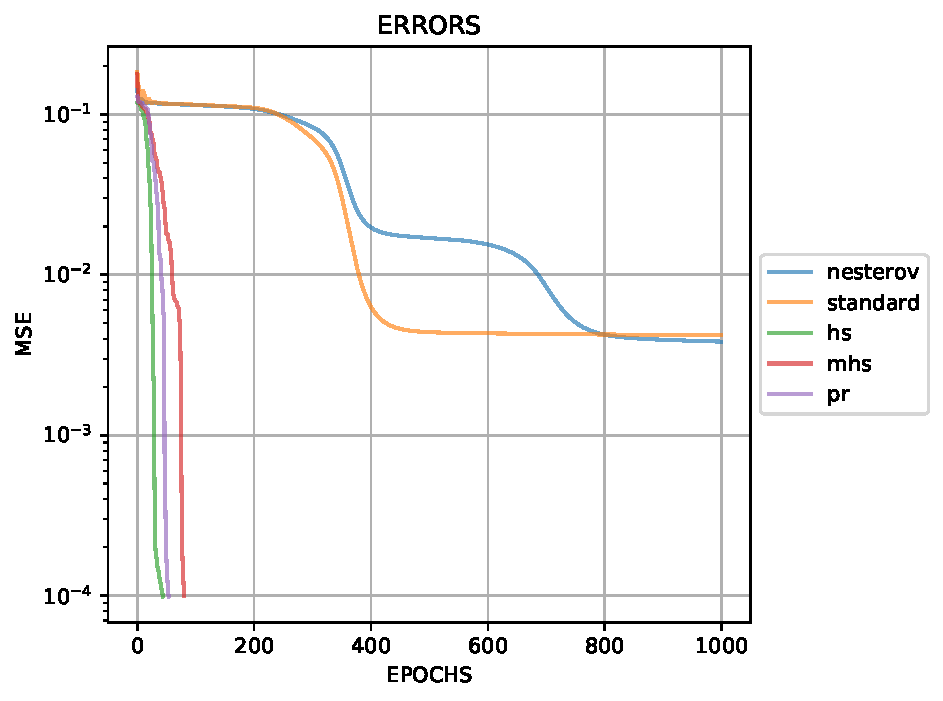
\includegraphics{img/comparisons/2_mse_all_max_epochs_1000.pdf}
                    }
                    \caption{}
                    \label{fig:monks_2_MSE_all_max_epochs}
                \end{subfigure}
                \begin{subfigure}{0.45\textwidth}
                    \resizebox{\textwidth}{!}{
                        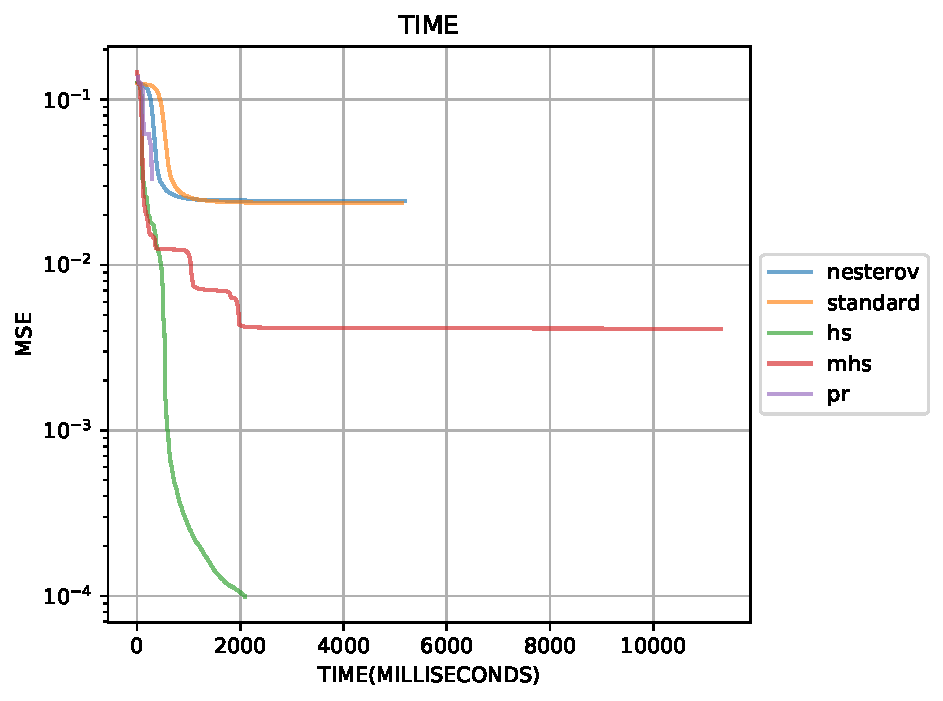
\includegraphics{img/comparisons/3_mse_all_time_max_epochs_1000.pdf}
                    }
                    \caption{}
                    \label{fig:monks_3_MSE_all_max_epochs_t}
                \end{subfigure}
                \begin{subfigure}{0.45\textwidth}
                    \resizebox{\textwidth}{!}{
                        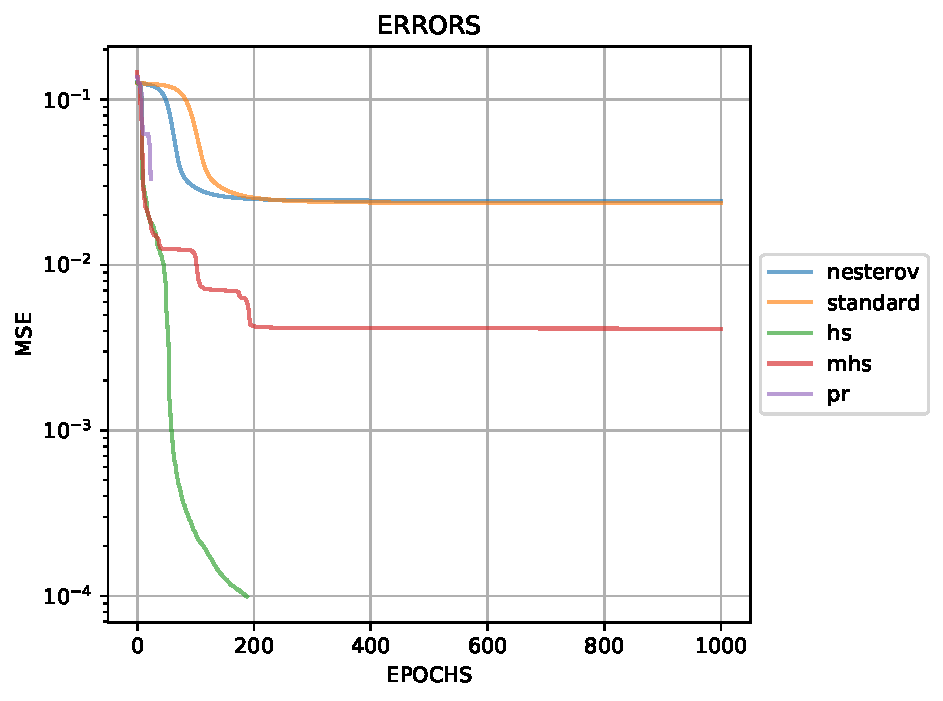
\includegraphics{img/comparisons/3_mse_all_max_epochs_1000.pdf}
                    }
                    \caption{}
                    \label{fig:monks_3_MSE_all_max_epochs}
                \end{subfigure}
                \caption{Comparisons between the different optimizers with the constrain of setting a
                maximal number of epochs egual to 1000. In Figure \ref{fig:monks_1_MSE_all_max_epochs}, \ref{fig:monks_1_MSE_all_max_epochs_t}
                we can see the comparison for MONKS 1, while in Figure \ref{fig:monks_2_MSE_all_max_epochs}, \ref{fig:monks_2_MSE_all_max_epochs_t}
                we can see the one for MONKS 2 and finally in Figure \ref{fig:monks_3_MSE_all_max_epochs}, \ref{fig:monks_3_MSE_all_max_epochs_t} we
                can see the one for MONKS 3.}
                \label{fig:monks_MSE_all_max_epochs}
            \end{figure}

        % subsection results_ (end)
    % section monks (end)

    % \section{CUP} % (fold)
    %     \label{sec:cup}

    %     A main difference with respect to the models used for Monk, is the choice of the topology of the Network.
    %     First of all, in this case, being the final task a regression one in which there are two different values to be predicted, the output layer of the ANN is composed by two neurons of output, each one associated to an identity function.

    %     Then, after some preliminary trials, we have decided to set the number of the hidden layers to $[16,\ 32]$.

    %     Of course, as for the Monk dataset, we have performed a validation phase on the CUP dataset, in order to
    %     discover the best parameters for the network. As described in Sec. \ref{sec:monks}, it has been
    %     implemented a \textit{3-fold cross validation algorithm} with a (random) \textit{grid search}.
    %     Table \ref{tab:hyper_cup} shows the ranges in which the searching of the hyperparameters has been carried
    %     out. Once again, the momentum type chosen is Nesterov, while the direction used in the Conjugate Gradient
    %     Methods is the modified one.

    %     \begin{table}[H]
    %       \centering
    %       \caption{Hyperparameters' ranges for the random grid search algorithm with SGD and CG.}
    %       \begin{minipage}{.4\textwidth}
    %           \centering
    %           \begin{tabular}{| c | c |}
    %                 \hline
    %                 Hyperparameters & Ranges\\
    %                 \hline
    %                 $\eta$ & $\left [0.004, 0.2\right ]$ \\
    %                 \hline
    %                 $\alpha$ & $[0.5, 0.9]$ \\
    %                 \hline
    %                 $\lambda$ & $[0.0003, 0.003]$ \\
    %                 \hline
    %           \end{tabular}
    %       \end{minipage}
    %       \begin{minipage}{.4\textwidth}
    %           \centering
    %           \begin{tabular}{| c | c |}
    %                 \hline
    %                 Hyperparameters & Ranges\\
    %                 \hline
    %                 $\sigma_2$ & $\left [0.1, 0.4 \right ]$\\
    %                 \hline
    %                 $\rho$ & $[0.0, 1.0]$ \\
    %                 \hline
    %           \end{tabular}
    %         \end{minipage}
    %         \label{tab:hyper_cup}
    %     \end{table}

    %     In tables \ref{tab:cup_sgd} and \ref{tab:cup_cgd} are annotated the average results obtained from 10 executions of each one of the best models identified thanks to the validation step.

    %     \begin{table}[H]
    %             \centering
    %             \begin{subtable}{\textwidth}
    %                 \resizebox{\textwidth}{!}{
    %                     \begin{tabular}{| c | c | c | c | c | c | c | c |}
    %                         \hline
    %                         Model & Topology & Batch size & Activation & $\eta$ & $\alpha$ & $\lambda$
    %                         & MSE (TR - TS) \\
    %                         \hline
    %                         SGD & 10 -> 16 -> 32 -> 2 & batch & identity & 0.084 & 0.79 & 0.0009 & 1.00 - 1.35 \\
    %                         \hline
    %                     \end{tabular}
    %                 }
    %             \end{subtable}
    %             \caption{Results for the Stochastic Gradient Descent.}
    %             \label{tab:cup_sgd}
    %     \end{table}

    %     \begin{table}[H]
    %             \centering
    %             \begin{subtable}{\textwidth}
    %                 \resizebox{\textwidth}{!}{
    %                     \begin{tabular}{| c | c | c | c | c | c | c | c |}
    %                         \hline
    %                         $\beta$ & Topology & Batch size & Activation & $\sigma_1$ & $\sigma_2$ & $\rho$
    %                         & MSE (TR - TS) \\
    %                         \hline
    %                         $MHS^+$ & 10 -> -> 16 -> 32 -> 2& batch & identity & 0.0001 & 0.27 & 0.29 & 0.97 - 1.50\\
    %                         \hline
    %                         $HS^+$  & 10 ->-> 16 -> 32 -> 2& batch & identity & 0.0001 & 0.39 & 0.0
    %                         & 0.97 - 1.50  \\
    %                         \hline
    %                         $PR^+$  & 10 ->-> 16 -> 32 -> 2& batch & identity & 0.0001 & 0.86 & 0.00
    %                         & 1.15 - 1.41\\
    %                         \hline
    %                     \end{tabular}
    %                 }
    %             \end{subtable}
    %             \caption{Results for the Conjugate Gradient Methods.}
    %             \label{tab:cup_cgd}
    %     \end{table}

    %     As for the experiments with the Monk datasets, we attach the learning curves in Appendix \ref{cha:cup_learning_curves}.
% chapter experiments (end)
